\chapter{\tool --补丁定位方法}

本章将详细阐述\tool --一种基于多源知识的开源软件漏洞的补丁识别方法的设计。

\section{方法概述}
\begin{figure*}[h]
    \centering
    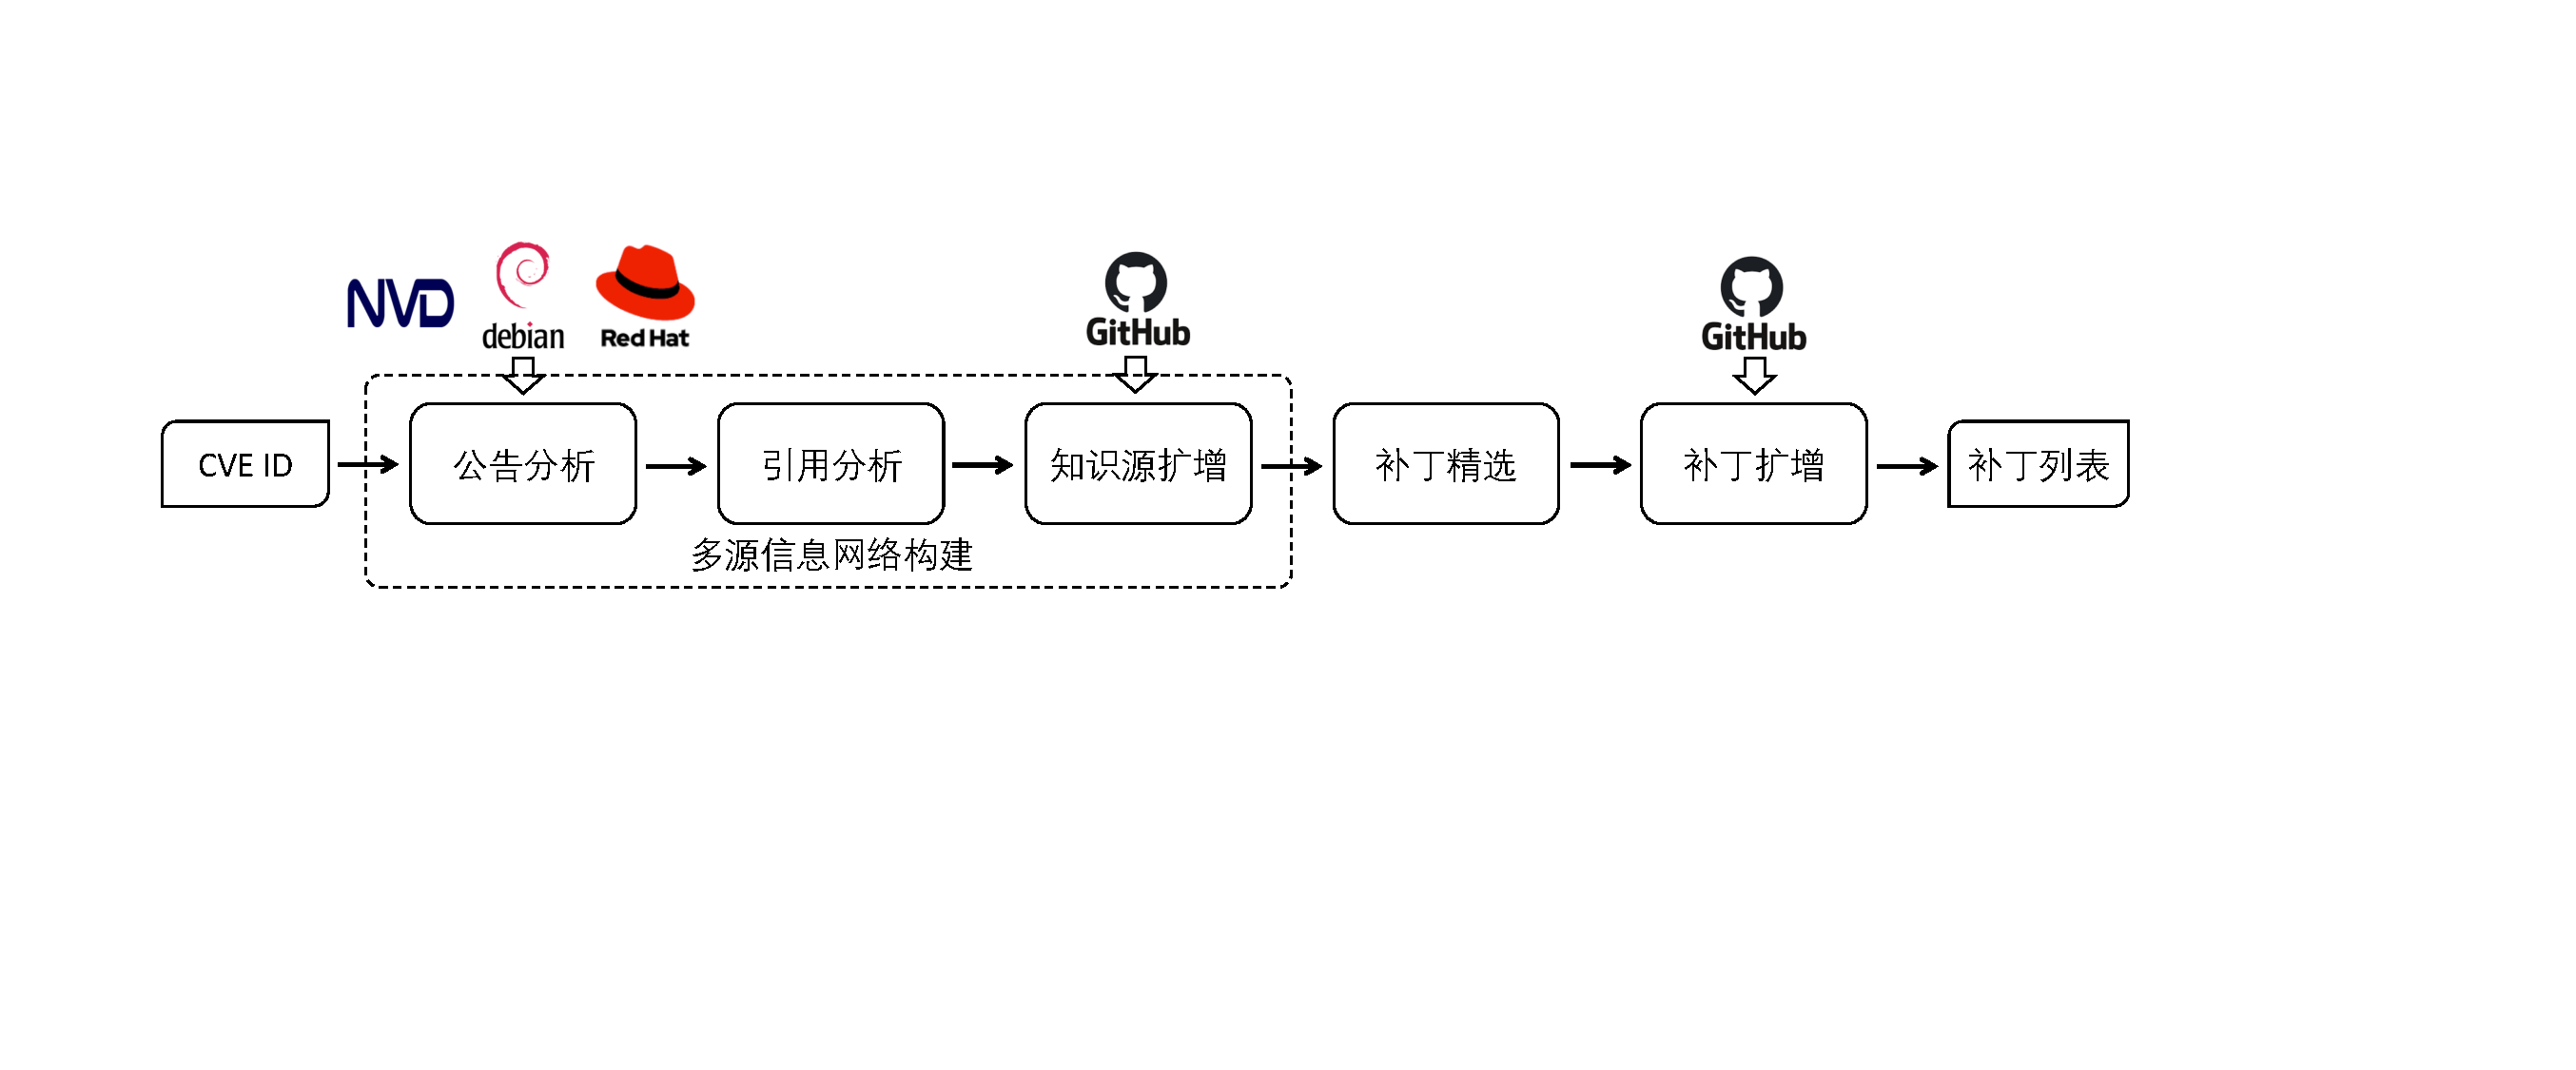
\includegraphics[scale=0.40]{res/overview.pdf}
    %\vspace{-10pt}
    \caption{\tool 方法概览}\label{fig:overview}
\end{figure*}

基于上文经验研究的发现,本文提出了一种名为\tool 的自动化方法来查找来源软件漏洞的补丁(Github Commit形式)。\tool 的基本思想是:漏洞的补丁信息(即:commit)会在与该漏洞相关的各种来源的漏洞公告、分析报告、讨论和解决的过程中被频繁提及和引用。

图\ref{fig:overview}展示了\tool 的方法概览。\tool 以漏洞的CVE标识符作为输入,最终返回其补丁信息。具体分为三步:首先,\tool 从多个\tocheck{信息源}(即:NVD、Debian\cite{debian}、RedHat\cite{redhat}和GitHub)为输入的CVE构建一个相关引用链接的信息网络。该步骤的目的是将CVE在报告、讨论和解决阶段的引用链接信息进行建模。这里将NVD视为主信息来源,将Debian、RedHat和GitHub视为次级信息来源,该级信息源可以进一步扩展。其次,\tool 从构建的参考链接网络中,选择中具有高连通性和高置信度的补丁节点(即:commit)作为该CVE的补丁。最后,\tool 通过搜索同一存储库中其他分支上的相关提交来扩展补丁集。该步骤目的是在CVE及其补丁之间建立潜在的一对多映射关系。在本章的其他小节中,将详细阐述每个步骤。

% \begin{itemize}[leftmargin=*]
% \item 首先,\tool 从多个\tocheck{信息源}(即:NVD、Debian\cite{debian}、RedHat\cite{redhat}和GitHub)为输入的CVE构建一个相关参考链接的网络。该步骤的目的是将CVE在报告、讨论和解决阶段的参考链接信息进行建模。这里将NVD视为主信息来源,将Debian、RedHat和GitHub视为次级信息来源,该级信息源可以进一步扩展。
% \item 其次,\tool 从构建的参考链接网络中,选择中具有高连通性和高置信度的补丁节点(即:commit)作为该CVE的补丁。
% \item 最后,\tool 通过搜索同一存储库中其他分支上的相关提交来扩展补丁集。该步骤目的是在CVE及其补丁之间建立潜在的一对多映射关系。
% \end{itemize}

\section{步骤一:构建多源引用信息网络}
\tool 的步骤一共包括三个子步骤,前两个子步骤为漏洞公告分析和引用分析,通过分析来自NVD、Debian和Red Hat三个信息源的漏洞公告构建初始引用信息网络;第三个子步骤为信息增强,通过从GitHub搜索相关提交链接来扩充信息网络。

\subsection{公告分析}
首先,\tool 初始化信息网络,将输入的CVE-ID设置为根节点,然后再添加三个漏洞公告源节点(即:NVD、Debian和Red Hat)作为root的子节点。这些公告源节点用于追溯最终选定的补丁节点的来源。

\begin{figure}[h]
    \centering
    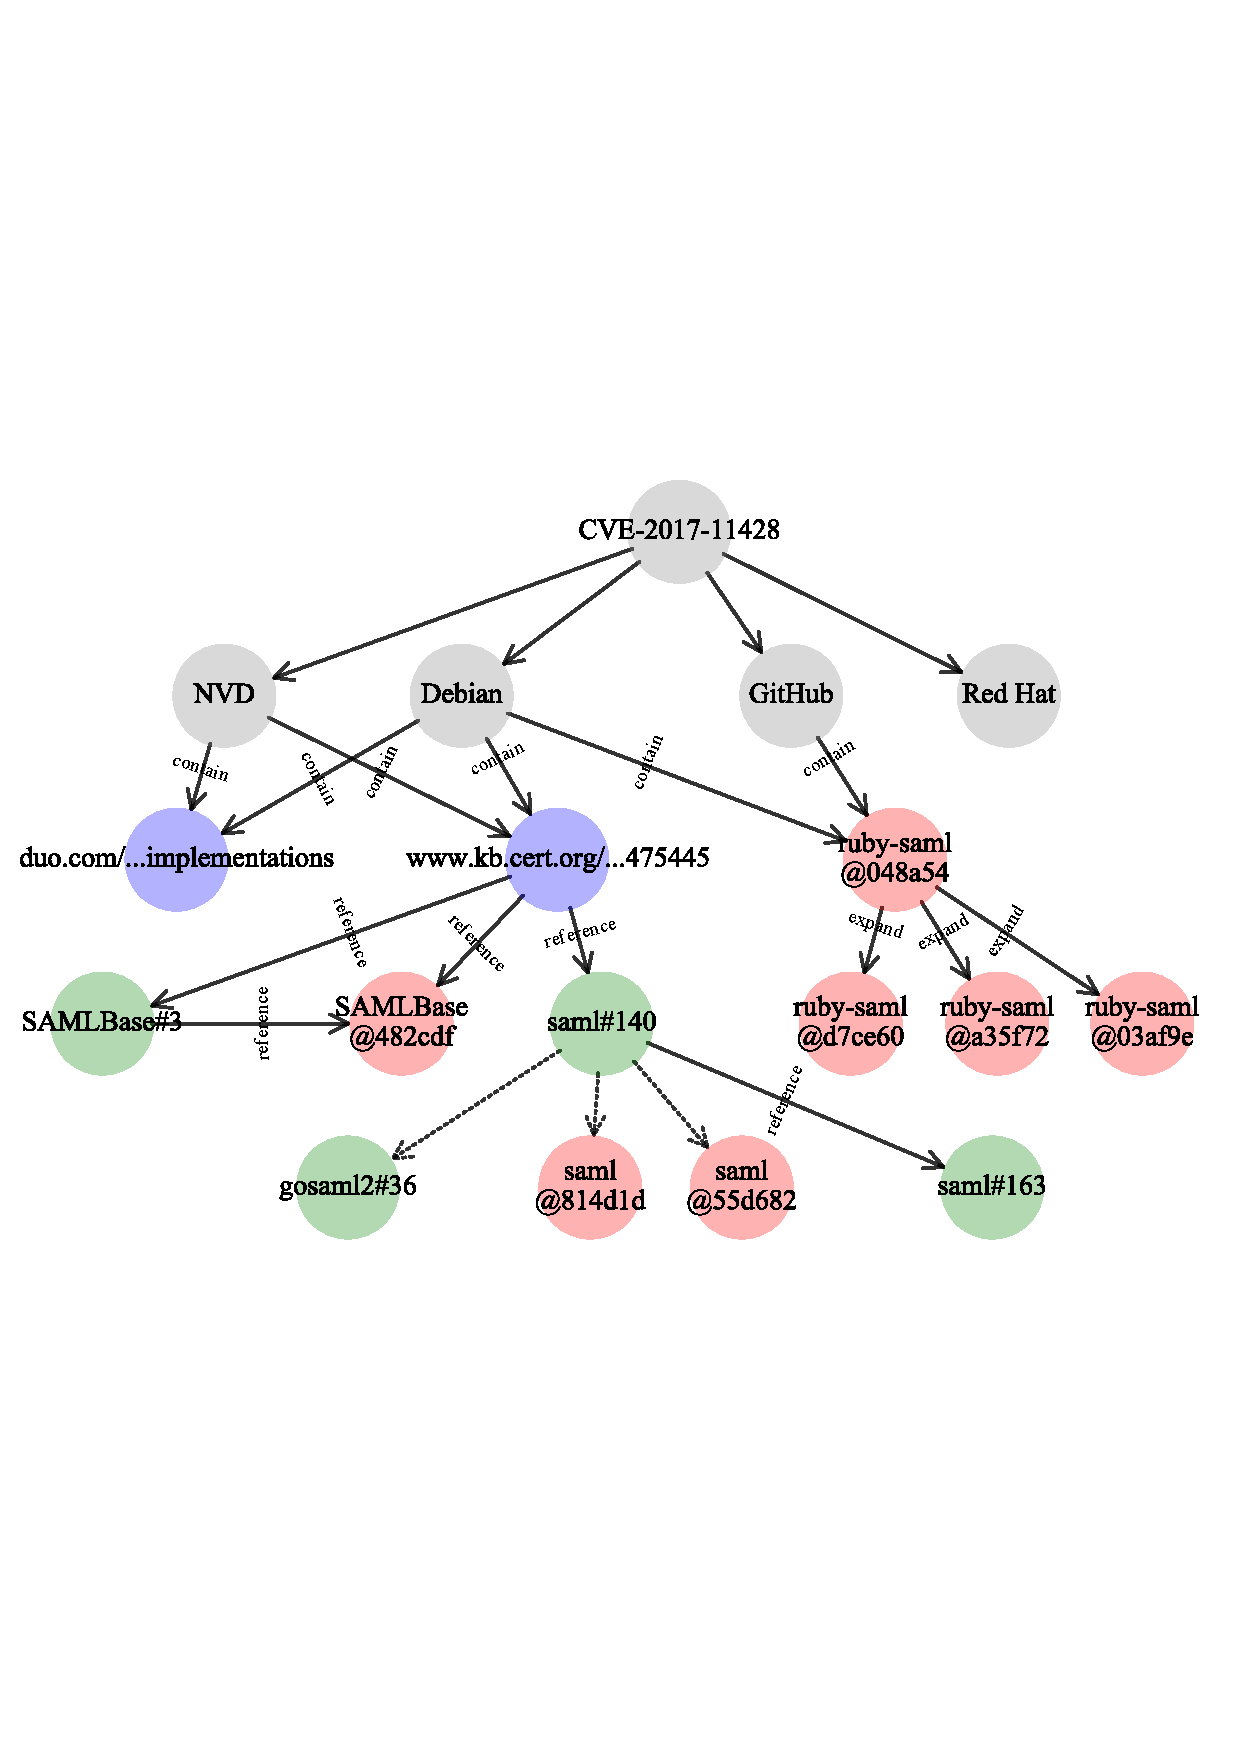
\includegraphics[scale=0.68]{res/network-example.pdf}
    %\vspace{-10pt}
    \caption{样例CVE-2017-11428的多源信息网络}\label{fig:example}
\end{figure}

\begin{exmp}
图\ref{fig:example}为样例CVE-2017-11428的完整的多源引用信息网络。 其中,顶层显示根节点,第二层显示公告来源节点。
\end{exmp}

然后,\tool 基于CVE-ID分别获取NVD、Debian和Red Hat的漏洞公告。其中,NVD平台以JSON形式按年份提供所有漏洞的结构化数据\cite{nvd-feed},\tool 通过下载并解析相应的JSON文件即可获得NVD中该CVE的信息。Debian平台的漏洞公告存储在仓库\cite{debian-repo}中,\tool 可直接从中解析得Debian提供的该CVE。Red Hat平台提供了 WebService API\cite{redhat-api}服务,\tool 可以直接使用该服务来检索Red Hat平台的漏洞公告。值得注意的是,分析发现:Debian会跟踪NVD上的所有CVE漏洞,而Red Hat仅会跟踪部分CVE漏洞。

\tool 从每个信息源的漏洞公告中提取引用信息(即:URL),并将它们添加为相应公告源节点的子节点。对于NVD公告,\tool 从“references”字段中提取出相关URL;类似地,对于Debian公告,\tool 会从“Notes”字段中提取出相关URL;对于Red Hat公告,\tool 使用正则表达式从评论区“comments”字段中提取出相关URL,这是因为开发人员会在评论区讨论和记录漏洞的解决过程,并可能列出对补丁信息。

\begin{exmp}
如图\ref{fig:example}中的第三层所示,对于CVE-2017-11428,NVD中包含了两个引用链接。链接一\tocheck{引用}是对描述此漏洞细节的博客的引用,链接一\tocheck{引用}是对该漏洞的第三方公告的引用。同时,这两个引用链接也包含在Debian公告中,不过该公告还包含对修复此漏洞的GitHub提交链接ruby-saml@048a54\cite{ruby-saml-1}的引用。此外,Red Hat平台并未收录该CVE。
\end{exmp}

\tool 将引用链接节点分为三种类型:补丁节点(Patch Node)、\tocheck{问题节点}(Issue Node)和\tocheck{混合节点}(Hybrid Node)。这里区分出补丁节点,是因为该方法的目标是为CVE找到补丁。区分出问题节点是因为开发人员常常会在问题追踪系统(Issue Tracker)中讨论该issue的解决方案并引用补丁链接信息;此外,问题追踪系统(Issue Tracker)中的报告会为CVE分配一个标识符(issue-id),开发人员常常会将issue-id写入补丁提交信息(即:commit message)中。未识别为补丁或问题节点的引用链接节点将被视为混合节点,它们多为博客、第三方漏洞公告等网页链接。

%受经验研究中补丁类型分析结果启发(Sec.\ref{sec:type}),
对于补丁节点的识别,如果URL链接中包含“git”字段且可通过正则表达式匹配到commit-id,则该链接为SVN commit形式的补丁节点;如果URL链接中包含“svn”字段且可通过正则表达式匹配到commit-id,则该链接为SVN commit形式的补丁节点。

对于问题节点的识别,如果URL链接中包含``/github.com/''和``/issues/'',则该链接为GitHub issue形式的问题节点;如果URL链接中包含``/github.com/''和``/pull/'',则该链接为GitHub pull request形式的问题节点;如果URL链接中包含``bugzilla"、``jira"、``issues"、``bugs"、``tickets"和``tracker"中的某一个字段且可通过正则表达式匹配到issue-id,\tocheck{则该链接为通常issue tracker形式的问题节点}。

\begin{exmp}
如图\ref{fig:example}中的第三层所示,NVD和Debian公告中包含的两个引用链接被标识为混合节点(即:图中的两个紫色节点),仅有一个在Debian公告中的引用链接被识别为补丁节点(即:图中的红色节点)。
\end{exmp}

\subsection{引用分析}

\subsection{信息增强}

\section{步骤二:精选补丁节点}

\section{步骤三:补丁扩增}